% =========================================================================
% HumanBrain Cross-Species CIS -- final journal-style manuscript (LaTeX)
% =========================================================================
% Scientific source of truth: frozen repository artifacts (v1.1.0 package).
% Every number below is quoted from audited frozen artifacts
% (RESOLUTION.md, e03_summary.json, e04b_summary.json, table_05/06/07/08/09,
% FIGURE_CAPTIONS.md, FINAL_RESEARCH_STATUS.md). Tables are AUTO-GENERATED
% from those artifacts by TABLE_SOURCES/generate_tables.py (fail-loud
% assertions); figures are frozen outputs plus one schematic (Fig. 2).
% No scientific value was changed, added, or optimized. 46/46 audit checks.
% =========================================================================
\documentclass[11pt,a4paper]{article}

\usepackage[T1]{fontenc}
\usepackage[utf8]{inputenc}
\usepackage{newtxtext,newtxmath}
\usepackage[margin=2.4cm]{geometry}
\usepackage{graphicx}
\usepackage{booktabs}
\usepackage{amsmath} % amssymb omitted: newtxmath provides AMS symbols
\usepackage{microtype}
\usepackage{xcolor}
\usepackage[font=small,labelfont=bf,justification=justified]{caption}
\usepackage{enumitem}
\usepackage{titlesec}
\usepackage[hidelinks,colorlinks=true,linkcolor=blue!50!black,citecolor=blue!50!black,urlcolor=blue!50!black]{hyperref}

\graphicspath{{figures/}}

\title{\bfseries Control-impact architecture of the human structural
connectome: degree dominance, a small near-universal residual, and a
cross-scale architectural comparison with the fly connectome}

\author{Harsha Vardhan Malipeddi\\[2pt]
\small Independent Researcher}
\date{}

\newcommand{\CIS}{\mathrm{CIS}}
\newcommand{\EG}{E(G)}

\begin{document}
\maketitle

\begin{abstract}
\noindent\textbf{Background.} Network communication in brain connectomes is
dominated by node degree, but whether any degree-independent component of
node-level control impact exists---and whether it is anatomically
structured---remains unresolved, because most node-removal analyses are
group-average, lack matched controls, and lack null-model arbitration.
\textbf{Gap.} No prior study, to our knowledge, has combined exact per-node
removal-based control impact with per-subject population-scale statistics,
degree/strength matching, degree-preserving null ensembles, and a
pre-registered cross-scale comparison. \textbf{Methods.} We computed the
exact Control Impact Score, $\CIS(i) = (\EG - E(G-i))/\EG$, for all 456~nodes
in each of 801 QC-pass subjects from the AOMIC-ID1000 structural-connectome
resource ($N=900$ acquired; 456-node 4S456 parcellation; SIFT streamline
weights; 15\% proportional threshold), with degree-matched controls
($\pm10\%$), 100 degree-preserving (Maslov--Sneppen) nulls per graph in two
batteries ($100\times100$ full-CIS; $200\times100$ top-50), BH-FDR node-level
inference, system-enrichment tests with two control levels, and a
9-configuration robustness ladder. \textbf{Results.} Top-50 CIS concentration
exceeded its degree-preserving null in 200/200 subjects (median
$z = 16.36$; two-sided sign $p = 1.24\times10^{-60}$). CIS was strongly
degree-related (median $\rho = 0.943$). A small degree-independent residual
was present in 778/801 subjects (sign $p = 2.6\times10^{-197}$;
Cliff's $\delta = 0.100$, 95\%~CI $[0.078, 0.129]$; median Wilcoxon
$p = 0.167$), and 43/456 nodes survived FDR ($q<.05$; max Stouffer
$z = 23.30$). Compared with the frozen fly (FAFB v783) study
($\delta = 0.0979$, itself not surviving its null ensemble), the human
architecture is concordant in effect size and degree dominance, while the
residual's anatomical identity diverges: visual systems hold 2\% of the human
top 50 versus 80\% visual-centrifugal in the fly; the pre-registered
system-enrichment gate was negative. \textbf{Interpretation.} Control-impact
architecture---a dominant degree component plus a small, near-universal
degree-independent residual---shows cross-scale architectural similarity
while the residual's anatomical identity diverges. No new biological
mechanism, homology, or system-specific claim is made.
\end{abstract}

\vspace{2pt}
\noindent\textbf{Keywords:} structural connectome; network neuroscience;
control impact; node removal; degree-preserving null model; population
analysis; cross-species comparison; global efficiency.

\section{Introduction}

Node-removal and efficiency-based analyses of human structural connectomes
are classical tools for quantifying node-level influence
\cite{alstott2009,crossley2014}, and hub and rich-club organization of the
human connectome is well documented \cite{vandenheuvel2011}. A persistent
confound, however, is node degree: raw comparisons of node importance are
dominated by how strongly a node is connected, so that observed
``importance'' can reflect degree alone. Matched controls and
degree-preserving null models are both required to separate these effects
\cite{maslov2002}; the decisive lesson of the present project's frozen
fly-connectome predecessor is that matched-pair significance can dissolve
entirely under degree-preserving null arbitration.

Whether a \emph{degree-independent} component of control impact exists at the
single-subject level, is reproducible across a population, and is anatomically
structured cannot be answered by group-average designs: averaging across
subjects destroys the per-subject variability that such a component would
need to be detected against. Network-controllability approaches
\cite{gu2015,betzel2016} address influence from a complementary, dynamical
perspective but do not provide per-subject removal-based rankings with null
arbitration; simulated-lesion studies either operate on group averages
\cite{alstott2009,crossley2014,yuehhsin2024} or use matched-mass rather than
degree-preserving nulls in an ageing framing \cite{kudriavtsev2026}.
Cross-species connectome comparisons \cite{venkadesh2025,yadav2025} and the
Amsterdam Open MRI Collection \cite{snoek2021} supply the comparative and
data foundations for the present design.

\textbf{Research question.} Can removal-based control impact identify
structurally influential nodes in individual human structural connectomes at
population scale, and does a degree-independent component of that impact
exist---and is it anatomically structured?

\textbf{Hypotheses (pre-registered in \texttt{PROTOCOL\_FREEZE.md} before any
computation).} \textbf{H1:} top-50 CIS concentration exceeds degree-preserving
null expectations. \textbf{H2:} a degree-independent residual remains after
degree/strength adjustment. \textbf{H3:} the residual is robustly
system-specific. \textbf{H4:} comparable architecture appears across fly and
human scales.

\textbf{Contribution.} To our knowledge, no prior study has combined
per-node removal-based network-impact analysis, population-scale individual
human structural connectomes, explicit degree-controlled residualization,
degree-preserving null-model arbitration, FDR-controlled residual inference,
and a pre-specified cross-species comparison with the \emph{Drosophila}
connectome in a single analytical framework. The novelty lies primarily in
this integration and the resulting cross-scale empirical comparison, not in
any individual component: each method is established
\cite{alstott2009,vandenheuvel2011,gu2015,betzel2016,maslov2002}.

\section{Methods}

\subsection{Study overview}
Figure~\ref{fig:workflow} summarizes the pipeline. All analyses were
pre-registered and frozen before outcome evaluation
(\texttt{PROTOCOL\_FREEZE.md}, \texttt{STUDY\_DESIGN.md}); every number in
this manuscript traces to a frozen artifact, and an independent stdlib-only
audit recomputes all documented values from those artifacts (46/46 checks;
\texttt{verify\_final\_numbers.py}).

\begin{figure}[!t]
\centering
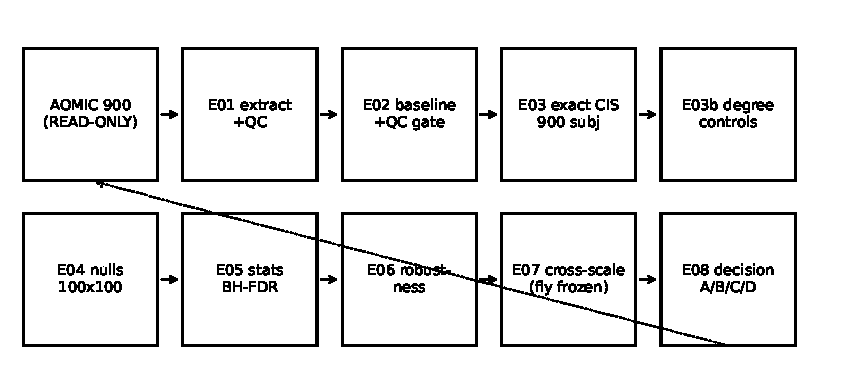
\includegraphics[width=\textwidth]{fig01_workflow.pdf}
\caption{\textbf{Study design and pipeline.} From the population-scale
AOMIC-ID1000 structural-connectome resource (900 subjects acquired; 801
QC-pass on frozen, CIS-blind flags), exact per-node Control Impact Scores
were computed for all 456 nodes in every subject, followed by degree-matched
controls ($\pm10\%$ total degree), degree-preserving (Maslov--Sneppen) null
ensembles in two batteries, BH-FDR node-level inference, two-level
system-enrichment tests, a 9-configuration robustness ladder, and a
pre-registered cross-scale comparison with the frozen fly (FAFB v783) study.}
\label{fig:workflow}
\end{figure}

\subsection{Dataset and cohort}
Structural connectomes were drawn from the AOMIC-ID1000 derivative
(Zenodo~19796783; CC-BY-4.0) \cite{snoek2021}: 900 subjects $\times$ 7 atlases
$\times$ 4 weight variants, checksum-verified on acquisition (10 archives,
7{,}067{,}175{,}601 bytes, byte-exact against the Zenodo API). The primary
configuration is 4S456Parcels ($N = 456$ nodes) with
\texttt{sift\_radius2\_count\_connectivity} weights at a 15\% proportional
threshold ($k = 15{,}561$ edges). Cohort membership was frozen from
pre-registered, CIS-blind, property-based QC (E02): 801/900 subjects pass
(94 isolated-node and 5 strength-IQR flags; flagged subjects retained, never
deleted). Thresholding keeps the $k = c\,N(N-1)/2$ largest off-diagonal
weights per graph (raw densities 0.45--0.88 preclude unthresholded
path-length statistics); the cost ladder $\{0.10, 0.20, 0.25\}$ is used for
robustness. Population baseline statistics are given in
Table~\ref{tab:cohort}.

% Auto-generated float (caption + label inside the file):
% AUTO-GENERATED from 09_TABLES/table_01_subject_cohort.csv -- do not edit numbers by hand.
\begin{table}[!t]
\centering\small
\caption{Primary cohort and baseline network properties. Structural connectomes
were extracted for 900 subjects; 801 pass the pre-registered, CIS-blind
property-based QC (flags retained, never deleted). Baseline statistics are for
the primary configuration (4S456Parcels, \texttt{sift\_radius2\_count} weights,
15\% proportional threshold). E0: global efficiency; $k$: mean degree.
Values are frozen artifact outputs (\texttt{table\_01\_subject\_cohort.csv},
\texttt{table\_03\_qc\_summary.csv}, \texttt{table\_02\_baseline\_network.csv}).}
\label{tab:cohort}
\begin{tabular}{lll}
\toprule
Quantity & Value & Source \\
\midrule
Subjects acquired & 900 & frozen manifest \\
QC-pass primary cohort & 801 ($0.89$) & E02 property QC \\
Flags retained (isolated-node / strength-IQR) & 94 / 5 & \texttt{qc\_primary.csv} \\
Parcellation (nodes $N$) & 4S456Parcels ($N=456$) & atlas manifest \\
Weight variant & \texttt{sift\_radius2\_count\_connectivity} & frozen config \\
Proportional threshold $c$ & 0.15 ($k=15{,}561$ edges) & E01 \\
Mean degree $\langle k\rangle$ & 68.2 & baseline artifact \\
Global efficiency $E_0$ (median) & 0.5468 [0.5441--0.5497] & baseline artifact \\
\bottomrule
\end{tabular}
\end{table}


\subsection{Control Impact Score}
For each subject graph $G$ and node $i$, the Control Impact Score is the
fraction of baseline global efficiency lost on exact removal of $i$:
\begin{equation}
\CIS(i) \;=\; \frac{\EG - E(G-i)}{\EG},
\qquad
E(G) \;=\; \frac{1}{N(N-1)} \sum_{\substack{u,v=1\\ u\neq v}}^{N}
\frac{1}{d(u,v)},
\label{eq:cis}
\end{equation}
where $d(u,v)$ is the graph shortest-path distance in the binary undirected
thresholded graph and $E(G-i)$ is evaluated on the induced $(N-1)$-node
subgraph with $(N-1)(N-2)$ normalization. All $456$ per-node values are
computed exactly (Dijkstra; scipy) per subject. The reference implementation
was validated against a naive implementation to $6.1\times10^{-16}$ relative
error; a boolean-matrix fast path used \emph{only} for null graphs is
equivalence-gated at $10^{-9}$ (max deviation $4\times10^{-16}$).
Figure~\ref{fig:cismethod} summarizes the measurement, control, and
arbitration logic; Fig.~\ref{fig:cisarch}(A) shows the population-mean CIS
architecture (maximum population-mean CIS $0.00462$ at node 414;
frozen value $0.0046246$).

\begin{figure}[!t]
\centering
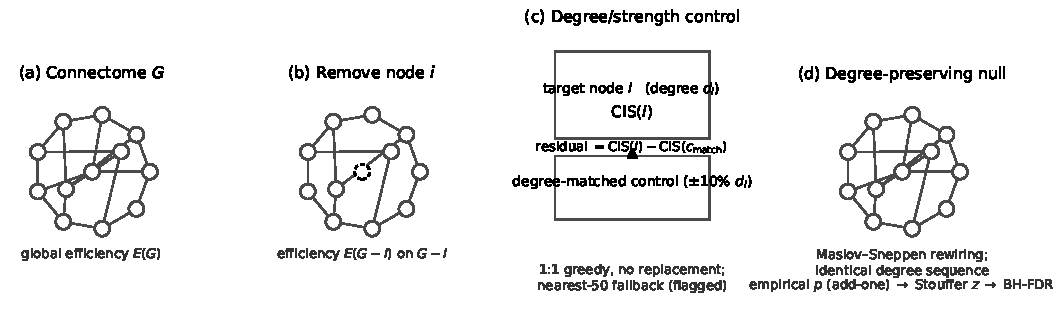
\includegraphics[width=\textwidth]{fig02_cis_method.pdf}
\caption{\textbf{CIS measurement, control, and arbitration (schematic; no
data plotted).} (a)~Baseline thresholded connectome $G$ with global
efficiency $\EG$ (Eq.~\ref{eq:cis}). (b)~Exact removal of node $i$ yields
$E(G-i)$ and $\CIS(i)$. (c)~Degree/strength control: each top-decile target
node is paired 1:1 with a $\pm10\%$-degree-matched control (greedy, no
replacement; nearest-50 fallback flagged per pair); the residual is
$\CIS(i) - \CIS(c_{\mathrm{match}})$. (d)~Arbitration: Maslov--Sneppen
rewiring preserves the exact per-node degree sequence; per-node empirical
$p$-values (add-one) feed Stouffer combination and BH-FDR, and per-subject
top-50 concentration is compared against its own null ensemble.}
\label{fig:cismethod}
\end{figure}

\subsection{Degree/strength controls and residual analysis}
Each top-decile CIS node is paired 1:1 with the nearest node within
$\pm10\%$ total degree (greedy, no replacement; nearest-50 fallback flagged),
yielding $36{,}846$ degree-matched pairs. The degree-independent residual is
\begin{equation}
r(i) \;=\; \CIS(i) - \CIS\!\left(c_{\mathrm{match}}(i)\right),
\label{eq:residual}
\end{equation}
summarized per subject by Cliff's delta
$\delta = \frac{\#\{(i,c):\, r(i) > 0\}}{N_{\mathrm{pairs}}}
        - \frac{\#\{(i,c):\, r(i) < 0\}}{N_{\mathrm{pairs}}}$.
The strength association is reported alongside
(median $\rho(\CIS,\text{strength}) = 0.486$ vs.\ $\rho(\CIS,\text{degree}) =
0.943$; Fig.~\ref{fig:cisarch}B).

\subsection{Degree-preserving nulls}
Null graphs are generated by undirected Maslov--Sneppen double-edge swaps
\cite{maslov2002} preserving the exact per-node degree sequence, with
$n_{\mathrm{swaps}} = 10\,|E|$ attempted swaps per null, rejection of
self-loops, duplicates, and degenerate picks, and exact per-null degree
verification ($10{,}000/10{,}000$ exact; 0 self-loops; swap acceptance
49.4\%). Two batteries: \textbf{battery A} (100 subjects $\times$ 100 nulls
$\times$ 456-node full-CIS recomputation) for per-node inference; and
\textbf{battery B} (200 subjects $\times$ 100 nulls of the top-50 median CIS;
100 fresh nulls plus 100 reused from battery A) for per-subject concentration.
Seeds are frozen (nulls $100+i$ per graph; subject samples nested under a
single RNG with seed 20260922; all recorded in
\texttt{null\_manifest\_battery\_a.csv}).

\subsection{Statistical inference}
\textbf{Battery B (H1):} per-subject $z$ against the null distribution of
the top-50 median CIS; population two-sided sign test.
\textbf{Battery A (R2a):} per-node one-sided empirical $p$ with the add-one
correction $p = (\#\{\text{nulls}\ge \text{obs}\}+1)/(100+1)$, Stouffer
combination $z_j = \sum_s z_{sj}/\sqrt{n_s}$, and Benjamini--Hochberg FDR at
$q = .05$ (single stratum). Censored nodes (all nulls $\ge$ observed; 413 of
456) carry $p=1$ and $z=-\infty$ by construction and are counted as censored,
not hidden. \textbf{System enrichment (H3/R2b):} control A = node-label
shuffle (10{,}000 permutations); control B = degree-matched peer pools
(10{,}000 resamples); $z$ and empirical $p$ with add-one floor.
\textbf{Rank stability:} 100 seeded half-splits, Spearman correlation of
mean-CIS ranks. \textbf{Effect sizes:} Cliff's $\delta$ with 95\% CIs.

\subsection{Cross-species comparison (pre-registered)}
The human analysis is compared with the frozen fly study (FAFB v783,
139{,}255 reconstructed neurons) using normalized comparators only, with
explicit discipline tags (DIRECT / NORMALIZED / QUALITATIVE; Table
\ref{tab:crossscale}). Human and fly nodes are not treated as homologous
structures; the comparison operates at the level of network architecture and
statistical organization across a $\sim$$10^{3}$-fold difference in analyzed
node count. Absolute CIS values are never compared across species.

\section{Results}

\subsection{Population CIS architecture and its degree relation}
CIS was computed for all 456 nodes in each of 801 subjects. The
population-mean CIS architecture is highly skewed
(Fig.~\ref{fig:cisarch}A): the maximum population-mean CIS is $0.00462$
(node 414), and node 400 falls in the per-subject top 50 in 100\% of
subjects. Small absolute magnitudes are expected at 15\% cost in a redundant
graph with mean degree $\langle k\rangle = 68.2$. CIS tracks degree far more
closely than strength (median Spearman $\rho = 0.943$ vs.\ $0.486$;
Fig.~\ref{fig:cisarch}B), motivating the degree-controlled residual analysis.
The highest-stability nodes are listed in supplementary Table~S1.

\begin{figure}[!t]
\centering
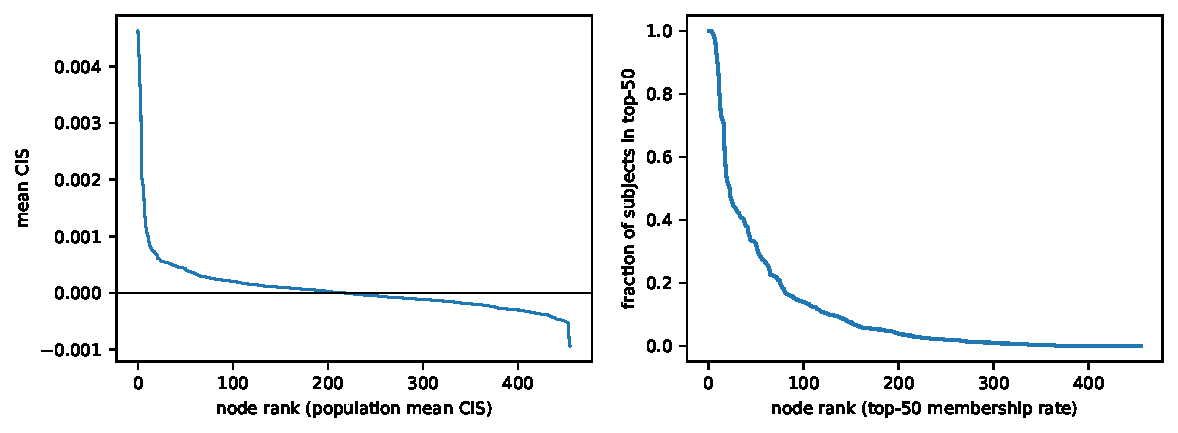
\includegraphics[width=\textwidth]{fig03_population_cis.pdf}\\[4pt]
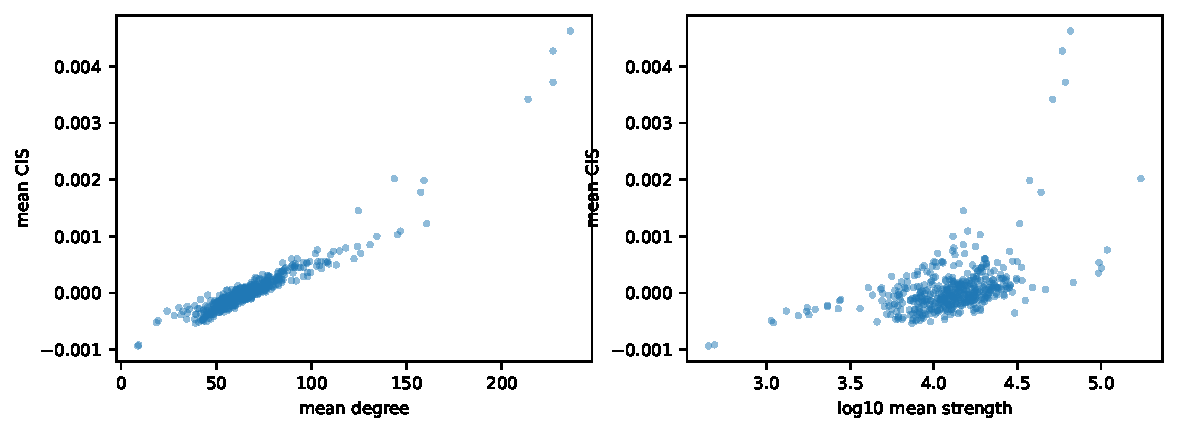
\includegraphics[width=\textwidth]{fig04_cis_vs_degree_strength.pdf}
\caption{\textbf{CIS architecture and its degree relation (801 subjects).}
\textbf{(A)} Population-mean CIS across all 456 nodes; CIS is unitless---the
fraction of baseline global efficiency $E(G)$ lost on node removal---with a
maximum population-mean CIS of 0.00462 (node 414). \textbf{(B)} CIS tracks
node degree (median Spearman $\rho = 0.943$) far more closely than strength
($\rho = 0.486$), motivating the degree-controlled residual analysis of
Fig.~\ref{fig:residual}.}
\label{fig:cisarch}
\end{figure}

\subsection{Degree-preserving null arbitration (H1)}
Top-50 CIS concentration exceeded its degree-preserving null in
\textbf{200/200 subjects} (median $z_{\mathrm{vs\,null}} = 16.36$; two-sided
sign $p = 1.24\times10^{-60}$; Fig.~\ref{fig:nulls}B). All per-subject
empirical $p$-values sit at the $1/101$ null-resolution floor; inference
therefore rests on the $z$ statistics and the population sign test, which we
state explicitly. Per-node Stouffer $z$ against battery A is finite for 43 of
456 nodes (maximum $23.30$ at node 400), with the remaining 413 nodes
censored at the empirical-$p$ floor (Fig.~\ref{fig:nulls}A).

\begin{figure}[!t]
\centering
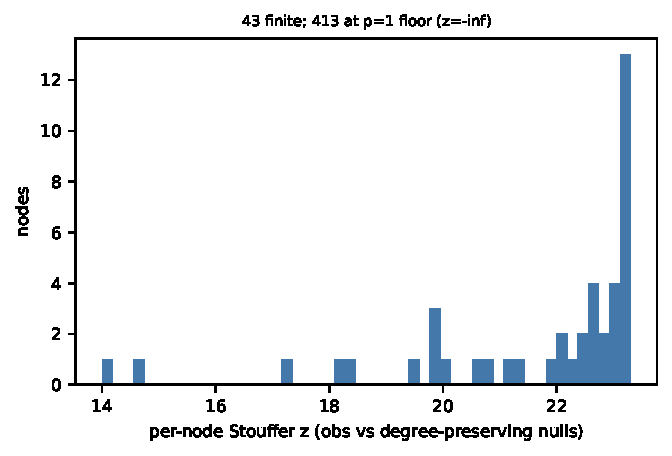
\includegraphics[width=0.62\textwidth]{fig06a_stouffer.pdf}\hfill
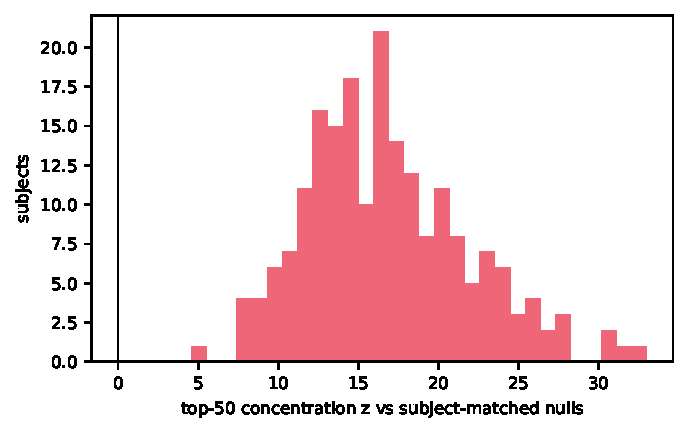
\includegraphics[width=0.36\textwidth]{fig06b_battery_b.pdf}
\caption{\textbf{Degree-preserving null arbitration.} \textbf{(A)} Per-node
Stouffer $z$ against the 100-null battery (battery A): 43 of 456 nodes carry
finite $z$ (maximum 23.30, node 400); the remaining 413 nodes sit at the
add-one empirical-$p$ floor and are explicitly counted as censored
($-\infty$), not hidden. \textbf{(B)} Per-subject top-50 concentration $z$
(battery B): all 200/200 subjects lie above their null ensembles. All
per-subject empirical $p$-values sit at the $1/101$ null-resolution floor;
inference therefore rests on the $z$ statistics and the population sign test
(two-sided $p = 1.24\times10^{-60}$).}
\label{fig:nulls}
\end{figure}

\subsection{Degree-independent residual (H2)}
The residual (Eq.~\ref{eq:residual}) is positive in \textbf{778/801 subjects}
(sign $p = 2.6\times10^{-197}$) with median Cliff's $\delta = 0.100$
(95\%~CI $[0.078, 0.129]$; IQR $0.078$--$0.129$ across subjects;
Fig.~\ref{fig:residual}). Of the $36{,}846$ individual matched comparisons,
58.8\% beat the control; the median paired Wilcoxon $p$ is $0.167$
(125/801 subjects $<.05$). The residual is therefore \emph{small in effect
size} but \emph{directionally near-universal across subjects}---measurable
only through matched controls plus null arbitration.

\begin{figure}[!t]
\centering
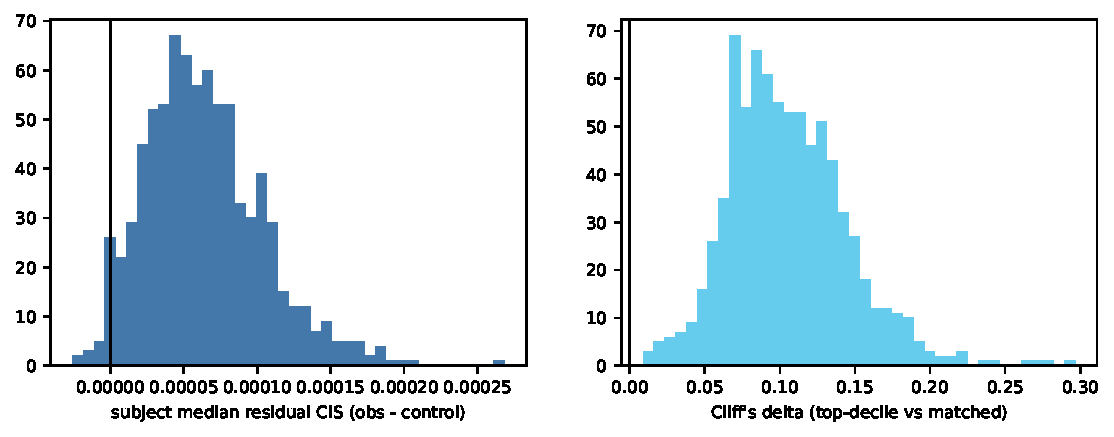
\includegraphics[width=\textwidth]{fig05_degree_controlled.pdf}
\caption{\textbf{Degree-independent residual architecture (801 subjects).}
Subject-median CIS residual against degree- and strength-matched controls
(36,846 pairs), and the per-subject Cliff's $\delta$ distribution: the
residual is positive in 778/801 subjects (sign $p = 2.6\times10^{-197}$) with
median $\delta = 0.100$ [IQR 0.078--0.129]; 58.8\% of individual matched
comparisons beat the control, and the median paired Wilcoxon $p$ is 0.167
--- small in effect size, directionally near-universal across subjects.}
\label{fig:residual}
\end{figure}

\subsection{Anatomical distribution and the pre-registered system gate
(H3/R2b)}
\textbf{43/456 nodes} survive BH-FDR $q<.05$ (maximum Stouffer $z = 23.30$,
node 400; cluster spanning nodes 400--451). Their anatomical distribution is
dominated by subcortical/cerebellar tissue (39 of 43), with limbic (2) and
default-mode (2) nodes (Fig.~\ref{fig:fdr}). The pre-registered
system-enrichment gate (R2b) was, however, \textbf{negative}: visual cortex
holds 1 of the top 50 (2\%; $z_B = -0.38$), and the single nominal system
signal (Subcortical/Cerebellar: observed 26, $z_A = 9.06$, $z_B = 2.08$,
$p = .031$, $1.25\times$) is absent at $K = 25$ ($z_B = 0.81$) and
degree-anchored. The four pre-specified sensory/attention systems show no
positive degree-matched enrichment (Table~\ref{tab:r2b}). H3 is therefore
\emph{not supported}: no robust canonical-system-specific explanation of the
residual was established.

\begin{figure}[!t]
\centering
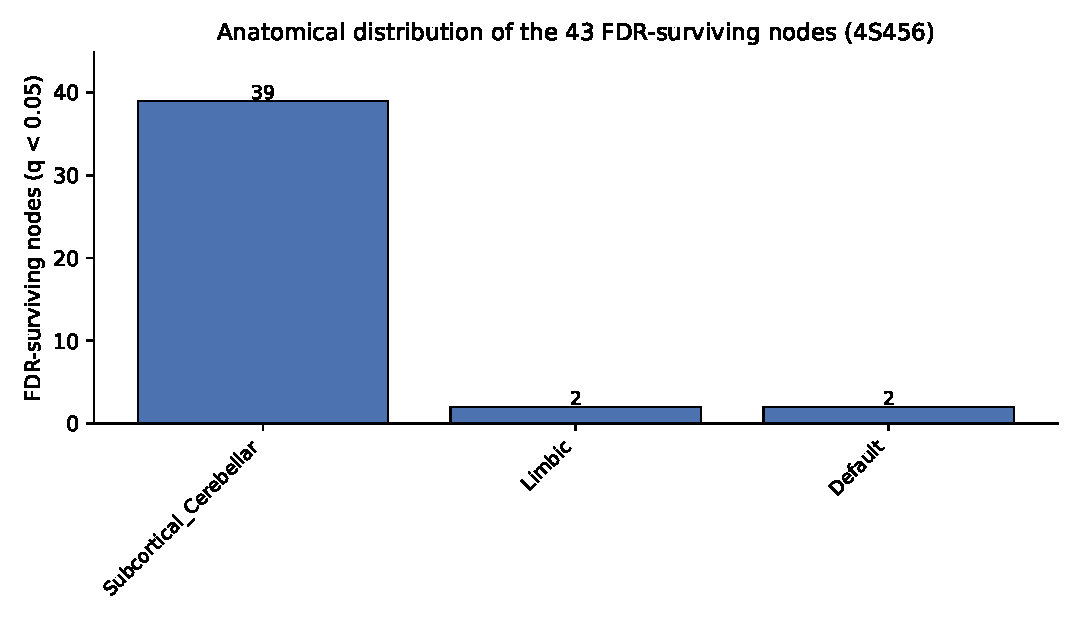
\includegraphics[width=0.82\textwidth]{fig05_fdr_anatomical.pdf}
\caption{\textbf{Anatomical distribution of the 43 FDR-surviving nodes.}
System counts of the 43/456 nodes surviving BH-FDR $q<.05$ (maximum Stouffer
$z = 23.30$): Subcortical/Cerebellar 39, Limbic 2, Default 2. The
pre-registered system-enrichment gate (R2b) itself was negative: visual
cortex holds 1 of the top 50 (2\%), and the single nominal system signal
(Subcortical/Cerebellar, $z_B = 2.08$, $p = .031$, $1.25\times$) is
degree-anchored and absent at $K = 25$. Rendered from the frozen
\texttt{table\_07\_null\_results.csv} plus the atlas label manifest; no
statistics were recomputed.}
\label{fig:fdr}
\end{figure}

% Auto-generated float (caption + label inside the file):
% AUTO-GENERATED from 10_REPORT/RESOLUTION.md R2b block -- do not edit numbers by hand.
\begin{table}[!t]
\centering\small
\caption{Pre-registered system-enrichment gate (R2b) at $K=50$ for the four
pre-specified sensory/attention systems: observed count in the top-50 residual
nodes, node-label-shuffle control ($z_A$, $p_A$; 10{,}000 permutations), and
degree-matched peer-pool control ($z_B$, $p_B$; 10{,}000 resamples), with
control-B enrichment. \textbf{The pre-registered gate was negative}: no
pre-specified sensory/visual system shows positive degree-matched enrichment
(Visual: 1/50 nodes, $z_B=-0.38$). The full eight-system table, including the
nominal Subcortical/Cerebellar signal ($z_B=2.08$, $p=.031$, $1.25\times$;
absent at $K=25$ and degree-anchored), is frozen in the E05 artifacts. Source:
\texttt{RESOLUTION.md} (verbatim).}
\label{tab:r2b}
\begin{tabular}{lcccccc}
\toprule
System & Obs. & $z_A$ & $p_A$ & $z_B$ & $p_B$ & Enrich.\ (B) \\
\midrule
Visual & 1 & -2.52 & 0.9995 & -0.38 & 0.7754 & 0.69x \\
Somatomotor & 2 & -2.59 & 0.9989 & -1.63 & 0.9813 & 0.38x \\
Dorsal attention & 3 & -1.03 & 0.9097 & -0.09 & 0.6296 & 0.96x \\
Salience/ventral attention & 8 & 1.40 & 0.1292 & -0.50 & 0.7524 & 0.86x \\
\bottomrule
\end{tabular}
\end{table}


\subsection{Robustness (E06)}
All nine pre-registered alternative configurations (atlases
\{4S256, 4S156, Brainnetome246Ext, AAL116\}; weights
\{\texttt{sift\_invnodevol}, \texttt{radius2\_count}\}; costs
$\{0.10, 0.20, 0.25\}$; frozen $n=150$ cohort, nested samples) reproduce the
primary architecture (Table~\ref{tab:robustness};
supplementary Fig.~S2). The maximum like-for-like top-50-mean deviation is
$0.00262$ (full precision $0.0026194$; atlas AAL116: $0.0038480$ vs.\ the
like-for-like primary $0.0012286$ on the same cohort). \emph{No numeric
tolerance was pre-registered for E06} in \texttt{PROTOCOL\_FREEZE.md} or
\texttt{STUDY\_DESIGN.md}; the concordance is a descriptive comparison, not a
pass/fail gate, and we report the exact deviation rather than a threshold
verdict. Rank stability across 100 half-splits is high (median Spearman
$0.996$, IQR $0.996$--$0.997$).

% Auto-generated float (caption + label inside the file):
% AUTO-GENERATED from 10_REPORT/RESOLUTION.md concordance block, cross-checked
% against 09_TABLES/table_08_robustness.csv -- do not edit numbers by hand.
\begin{table}[!t]
\centering\small
\caption{E06 robustness ladder: nine pre-registered alternative configurations
(frozen $n=150$ cohort, nested samples). Each condition reproduces the primary
architecture. $\Delta_{50}$: like-for-like deviation of the top-50 mean-of-means
from the like-for-like primary row (4S456, \texttt{radius2\_count}, cost 0.15,
same cohort; primary top-50 mean 0.0012286). $\ast$: maximum absolute
deviation, full precision $0.0026194$ (atlas AAL116: 0.0038480 vs 0.0012286).
No numeric tolerance was pre-registered for E06 in PROTOCOL\_FREEZE or
STUDY\_DESIGN; the concordance is a descriptive comparison, not a pass/fail
gate. Sources: \texttt{RESOLUTION.md}; \texttt{table\_08\_robustness.csv}.}
\label{tab:robustness}
\begin{tabular}{lcccccc}
\toprule
Condition & $n$ & top-50 mean & $\Delta_{50}$ & Gini (med.) & $\Delta$ Gini & $\rho$(CIS, deg.) (med.) \\
\midrule
cost 0.10 & 150 & 0.001564 & 0.000335 & 0.52647 & 0.03486 & 0.8978 \\
cost 0.20 & 150 & 0.001029 & -0.000200 & 0.47547 & -0.01614 & 0.9791 \\
cost 0.25 & 150 & 0.000926 & -0.000302 & 0.45767 & -0.03395 & 0.9950 \\
atlas 4S256 & 150 & 0.001887 & 0.000658 & 0.50955 & 0.01794 & 0.9422 \\
atlas 4S156 & 150 & 0.003179 & 0.001951 & 0.56178 & 0.07017 & 0.9566 \\
atlas Brainnetome246Ext & 150 & 0.001704 & 0.000476 & 0.45887 & -0.03274 & 0.9463 \\
atlas AAL116 & 150 & 0.003848 & 0.002619$\ast$ & 0.53892 & 0.04731 & 0.9447 \\
weights \texttt{sift\_invnodevol} & 150 & 0.001187 & -0.000042 & 0.48316 & -0.00845 & 0.9379 \\
weights \texttt{radius2\_count} & 150 & 0.001254 & 0.000026 & 0.48526 & -0.00635 & 0.9489 \\
\bottomrule
\end{tabular}
\end{table}


\subsection{Cross-scale comparison (H4)}
Table~\ref{tab:crossscale} and Fig.~\ref{fig:crossscale} give the
pre-registered comparators. The human residual effect size
($\delta = 0.100$) and the fly value ($\delta = 0.0979$) are concordant, and
both architectures are degree-dominated. Two boundaries must be stated with
the result. First, the fly $\delta$ \emph{did not survive} its own
degree-preserving null ensemble ($p = 0.109$); the cross-scale $\delta$
agreement is interesting but partly fortuitous (different units of analysis,
graphs, and designs). Second, the residual's anatomical identity diverges:
visual systems hold 2\% of the human top 50 versus 80\%
visual-centrifugal nodes in the fly top 50, and the fly visual-centrifugal
enrichment ($2.63\times$ after degree matching, $z_B = 5.30$,
$p \approx 10^{-4}$; 13/50 matched peers) has no positive human analog
(R2b negative). The comparison supports an architectural statement
only: \emph{architecture replicates; anatomy does not}.

% Auto-generated float (caption + label inside the file):
% AUTO-GENERATED from 07_CROSS_SCALE/table_09_cross_scale.csv -- do not edit numbers by hand.
\begin{table}[!t]
\centering\small
\caption{Pre-registered cross-scale comparators (human vs.\ fly), normalized
per the frozen discipline tags (DIRECT: same statistic and control design;
NORMALIZED: scale-normalized analogue; QUALITATIVE). Absolute CIS values are
never compared across species (different units, graphs, and designs). The fly
$\delta$ did not survive its own degree-preserving null ensemble ($p=0.109$).
Human and fly nodes are not treated as homologous structures; the comparison
operates at the level of network architecture and statistical organization.
Source: \texttt{table\_09\_cross\_scale.csv} (verbatim).}
\label{tab:crossscale}
\begin{tabular}{p{3.4cm}p{3.9cm}p{4.6cm}l}
\toprule
Comparator & Fly (FAFB v783) & Human (AOMIC-ID1000) & Tag \\
\midrule
Effect size of the CIS shift (target vs.\ matched controls), Cliff's $\delta$ & Cliff's delta = 0.0979 & Cliff's delta = 0.100 (median across 801 subjects; residual CIS vs degree-matched controls) & DIRECT \\
Null survival of the group-level CIS effect (degree-preserving ensembles) & z = 1.21, p = 0.109 (NOT survived) & battery B (E04b/E05): see NULL\_MODEL\_REPORT; top-50 median vs 100 degree-preserving nulls & DIRECT \\
Top-$K$ enrichment vs.\ tested universe (control A: label shuffle) & K=50 visual\_centrifugal: obs 21, enrich 11.7x, z\_A = 14.5 & E05 system enrichment z\_A per system & NORMALIZED \\
Top-$K$ enrichment vs.\ degree-matched expectation (control B) & K=50: E\_B 8.0, enrich 2.63x, z\_B = 5.30, p ~1e-4 & E05 z\_B per system (degree-matched peer pools) & DIRECT \\
Chokepoint catalogue depth & 50 nodes catalogued; 13 A\_strong\_chokepoint & top-100 catalogue (human\_chokepoint\_catalogue.csv); A/B classing pending E05 q-values & QUALITATIVE \\
Visual-system share of the top 50 & 80\% (visual\_system\_fraction\_top50, e14\_v2\_summary) & 2\% of top-50 nodes in Vis systems & DIRECT \\
\bottomrule
\end{tabular}
\end{table}


\begin{figure}[!t]
\centering
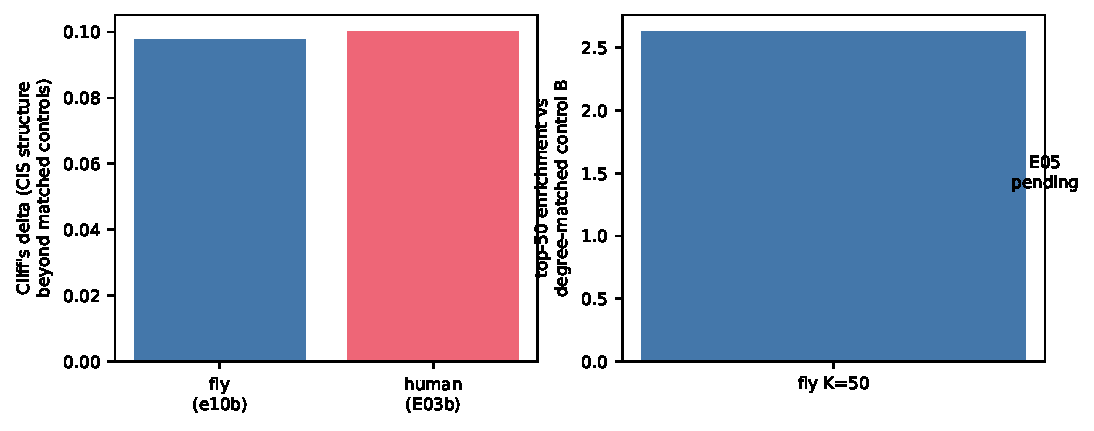
\includegraphics[width=\textwidth]{fig08_cross_scale.pdf}
\caption{\textbf{Cross-scale comparison (human vs.\ fly), normalized
comparators only.} Effect-size (Cliff's $\delta$), enrichment ($z_B$), and
concentration comparators, normalized per the cross-scale discipline tags:
human $\delta = 0.100$ vs.\ fly $\delta = 0.0979$ (the fly value did not
survive its own degree-preserving null ensemble, $p = 0.109$); human visual
share of the top 50 is 2\% versus 80\% visual-centrifugal in the fly.
Absolute CIS values are never compared across species (different units,
graphs, and designs).}
\label{fig:crossscale}
\end{figure}

\subsection{Hypothesis outcomes}
H1 \textbf{supported} (200/200; $z = 16.36$; $p = 1.24\times10^{-60}$);
H2 \textbf{supported} (778/801; $\delta = 0.100$; 43/456 FDR);
H3 \textbf{not supported} (R2b negative; nominal subcortical signal
degree-anchored and K-ladder-fragile); H4 \textbf{resolved as bounded
architectural concordance with anatomical divergence} (Table
\ref{tab:crossscale}; fly $\delta$ not null-surviving). These outcomes match
the frozen decision summary (\texttt{table\_10\_decision\_summary.csv}).

\section{Discussion}

\subsection{Principal findings}
Across 801 individual human structural connectomes, structural network
impact decomposes into a dominant connectivity-dependent component and a
smaller degree-independent residual: top-50 concentration exceeds
degree-preserving null expectations in every tested subject, the residual is
directionally near-universal ($778/801$; $\delta = 0.100$), and 43/456 nodes
survive FDR. The strong CIS--degree coupling ($\rho \approx 0.94$) replicates
the known degree--importance relationship \cite{alstott2009,crossley2014}
at population scale, now with per-subject resolution.

\subsection{The degree-independent residual}
The residual is small ($\delta = 0.100$; 58.8\% of matched pairs; median
Wilcoxon $p = 0.167$) and lies near the CIS noise floor; it is detectable
only through the combination of matched controls and null arbitration. Its
per-node structure is concentrated (43 nodes; max Stouffer $z = 23.30$), but
its system-level interpretation is negative (R2b). Matched-pair significance
without null arbitration can mislead---the fly study's GABA-specific
hypothesis, rejected here as a preserved negative result, is the canonical
demonstration.

\subsection{Cross-scale architecture}
A qualitatively similar two-component organization appears at both scales
despite a $\sim$$10^{3}$-fold difference in analyzed node count and
non-homologous anatomy. The relation to previous literature is bounded:
classical removal analyses \cite{alstott2009,crossley2014,yuehhsin2024} are
group-average without matched controls or nulls; the closest neighbour
\cite{kudriavtsev2026} uses matched-mass nulls in an ageing framing (partial
overlap; full-text verified); controllability studies
\cite{gu2015,betzel2016} address a complementary metric; cross-species
connectome analyses \cite{venkadesh2025,yadav2025} do not perform
per-node removal rankings with degree-matched controls and degree-preserving
nulls on both scales. These results motivate the hypothesis that
two-component control-impact organization may recur across nervous systems
of very different scale; they do not establish anatomical homology, a
conserved biological mechanism, or a universal law.

\subsection{Negative and null findings}
The following are first-class outcomes of this study, preserved as such:
(1)~the pre-registered human system-specific gate (R2b) was negative---no
pre-specified sensory/visual system is enriched in the residual, and the
single nominal subcortical/cerebellar signal ($z_B = 2.08$, $p = .031$) is
absent at $K=25$ and degree-anchored; (2)~the fly GABA-specific hypothesis
was rejected---the raw matched-pair effect ($\delta = 0.111$,
$p = 0.0011$) did not survive the degree-preserving null ensemble (observed
$\delta = 0.098$ vs.\ null $0.071 \pm 0.022$; empirical $p = 0.109$;
median-difference $p = 0.782$; $z = 1.21$); (3)~the fly residual effect size
itself is not null-surviving ($p = 0.109$); (4)~battery-B per-subject
empirical $p$-values do not resolve the tail ($1/101$ floor); (5)~the
subcortical residual is not robust across the pre-registered $K$ ladder, and
its FDR cluster overlaps the same node block as the nominal enrichment, so
R2a and R2b are not independent confirmations; (6)~no causal, homology,
mechanism, or universal-law claim is made at any point.

\subsection{Limitations}
This is an observational, secondary analysis of a single acquisition and
pipeline; graphs are undirected (directed variants are impossible in these
derivatives); results are atlas- and threshold-dependent in detail (though
robust across the 9-configuration ladder in architecture); the residual is
near the CIS noise floor, hence the two-layer control design; per-subject
empirical $p$-values are limited by the 100-null resolution; the subcortical
residual is not robust across the $K$ ladder; the literature audit cannot
exclude occupation of the analyzed combination in sources not surfaced by
the queries used; and the environment manifest for the frozen runs has a
disclosed provenance gap. No anatomical homology mapping, functional
equivalence, causal inference, or universal-law claim is made or supported.

\subsection{Conclusion}
Top-50 control-impact concentration exceeds degree-preserving null
expectations in every tested human subject; a small degree-independent
residual is present in 778/801 subjects and is not robustly system-specific;
and the cross-scale comparison with the fly connectome shows concordant
effect-size architecture with divergent anatomical identity. Architecture
replicates; anatomy does not. The finding is hypothesis-generating, and the
two-layer arbitration design (degree-matched controls plus degree-preserving
nulls) is the methodological prerequisite for testing it on future
connectomes.

\section{Data and code availability}
Data: AOMIC-ID1000 (Zenodo~19796783; CC-BY-4.0) \cite{snoek2021}. Fly
reference: frozen release v1.0.0 artifacts (read-only; FAFB v783, CC BY-NC
4.0). Raw data are not redistributed by this project; third-party datasets
retain their original licensing and usage terms. All human-side code,
manifests, validation reports, and append-only logs are available at
\url{https://github.com/harsha-vardhan-2006/humanbrain_cross_species_cis};
every number traces to an artifact
(\texttt{FINAL\_REPRODUCIBILITY\_AUDIT.md}), and the full numeric audit runs
without any recomputation via \texttt{verify\_final\_numbers.py}
(stdlib-only; 46/46 checks).

\section*{Author contributions (CRediT)}
\textbf{H.V.M.:} Conceptualization; Methodology; Software; Validation;
Formal analysis; Investigation; Data curation; Writing --- original draft;
Writing --- review \& editing; Visualization; Supervision; Project
administration. Funding acquisition: not applicable --- no external funding
was received or sought.

\section*{Conflict of interest}
The author declares no competing interests. The project used an AI coding
agent (Codebuff) for computational assistance under author supervision---a
methodological disclosure, not a competing interest; all scientific judgment
and responsibility remain with the author (repository research logs).

\section*{Ethics statement}
This study is a secondary analysis of publicly distributed,
already-published data (AOMIC-ID1000, Zenodo~19796783, CC-BY-4.0; FAFB v783,
CC BY-NC 4.0). No new human data were collected; per the author's
determination of 2026-09-26, no IRB approval or exemption is required for
this secondary use.

\section*{Acknowledgment of limitations of reproduction}
The frozen analysis environment (Python~3.13, numpy~2.4.2, scipy~1.18.0,
pandas~2.3.3) is recorded in \texttt{ANALYSIS\_FREEZE.md}; the environment
manifest for the original runs has a disclosed provenance gap. All reported
values are independently recomputable from frozen artifacts via the
repository audit script.

\bibliographystyle{unsrt}
\bibliography{references}

\end{document}
